\subsection{Models}

\begin{figure}[htb]
    \centering
    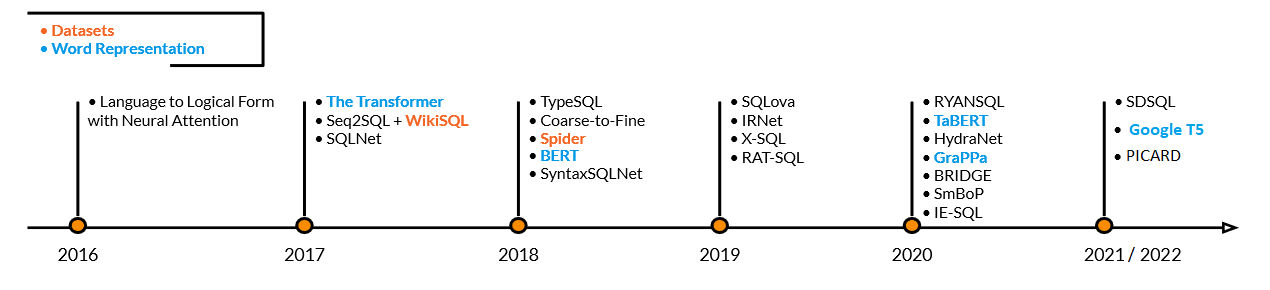
\includegraphics[width=0.99\textwidth]{pics/Timeline.png}
    \caption{An overview of the deep learning process for Text-to-SQL.}
    \label{fig:timeline}
\end{figure}

An efficient text-to-SQL solution requires state-of-the-art natural language processing techniques.
As a result of the neural network's ability to handle only numerical inputs and not raw text, word embedding has been used to represent numerical words.

Aside from that, in the past few years, language models have become increasingly popular as a solution for increasing performance in natural language processing tasks.

Assuming that words have numerical representations that differ from those of other words, word embeddings aim to map each word to a multidimensional vector, incorporating valuable information about the word. In addition to the brute-force creation of one-hot embeddings, researchers have developed highly efficient methods for creating representations that convey a word's meaning and relationships with other words. In most, if not all, Text-to-SQL systems, word embedding techniques such as Word2Vec\cite{DBLP:journals/corr/Rong14}, GloVe, and WordPiece embeddings\cite{DBLP:journals/corr/WuSCLNMKCGMKSJL16} are used.

Recently Language models have been shown to excel at NL tasks as a new type of pre-trained neural network. It is important to note that language models are not a replacement for word embeddings since they are neural networks and need a way to transform words into vectors.

Depending on the specific problem they want to solve, researchers can adapt the pre-trained model's inputs and outputs and train it for an additional number of epochs on their dataset. Thus, we can achieve state-of-the-art performance without complex architectures \cite{DBLP:journals/corr/abs-1810-04805}. Recent neural network architectures, like the Transformer\cite{DBLP:journals/corr/VaswaniSPUJGKP17}, have been used to achieve such performance by these models, which excel at handling NL and sequences of NL that are characterized by connections between words. Several language models have been used to handle the text-to-SQL task, including BERT \cite{DBLP:journals/corr/abs-1810-04805} and MT-DNN \cite{DBLP:journals/corr/abs-1901-11504}, while new models pre-trained specifically for structured data tasks are emerging, such as TaBERT\cite{DBLP:journals/corr/abs-2005-08314} and GraPPa \cite{DBLP:journals/corr/abs-2009-13845}.

% Furthermore, Text-to-SQL models and techniques represented in the SPIDER challenge will be studied and evaluated. 
The research section will assess the best state-of-the-art research in this field, starting from Seq2SQL\cite{zhong_seq2sql_2017} study in 2017 with the hype in WikiSQL challange and we will continue with SQLova\cite{hwang_comprehensive_2019} SQLNet\cite{xu_sqlnet_2017} and indtroduction of transformers and BERT with focus on RAT-SQL\cite{wang_rat-sql_2021} (2019), BRIDGE\cite{lin_bridging_2020} with BERT, HydraNet\cite{lyu_hybrid_2020} (2020), and the most recent solution with Google T5\cite{raffel_exploring_2020}, PICARD\cite{scholak_picard_2021} in SPIDER (2021).

% ////////////////////////////////////////////////////////////////////////////////

After reviewing the research papers on these models, we will study the implementation steps of these models. Moreover, evaluation methods and approaches to compare these models in accuracy for different datasets and if they are usable and reliable enough for our usage.

Most of these studies have excellent documentation regarding their implantation. Execution of these studies will be documented and published on Github. Nonetheless, In case of old and impractical implementation instructions, we will skip the implementation and continue with the top models available.

\subsection*{Seq2SQL}

An output of a sequence-to-sequence approach is a sequence of SQL tokens and schema elements, with that sequence being used to predict SQL queries or at least a significant portion of them. An NLQ sequence is transformed into a SQL sequence by these programs. There is no doubt that this approach is the simplest, but it is also the most error-prone. Seq2SQL\cite{zhong_seq2sql_2017}, one of the first deep-learning systems, used this approach, but later, systems avoided it. sequence-to-sequence architectures have the major disadvantage of not taking the strict grammar rules of SQL into account when generating queries.

As part of this model, its authors released the WikiSQL dataset, which ushered in a new era of text-to-SQL deep learning research. GloVe embeddings represent the inputs in the network architecture, which combines LSTM and linear layers. With a seq-to-seq network, the system predicts the aggregation function and the column for the SELECT clause. Its major drawback is that it generates parts of the query that can lead to syntactic errors.
\subsection*{SQLNet}
% cite Lin, Kevin, et al. “Grammar-based neural text-to-SQL generation.” arXiv preprint arXiv:1905.13326 (2019).

\begin{itemize}
    \item The model was designed to demonstrate that reinforcement learning should be limited in Text2SQL tasks.
    \item Until SQLNet, all previous models used reinforcement learning to improve the decoder results when it generated appropriate serializations.
    \item In cases where order is irrelevant, SQLNet avoids the seq2seq structure.
    \item For making predictions, the model uses a sketch-based approach consisting of a dependency graph that allows previous predictions to be taken into account.
    \item To improve the results, the model also incorporates column attention (weights assigned to significant words and phrases in sentences).
    \item According to the flowchart below, SQLNet employs three phases to generate SQL queries for WikiSQL tasks.
\end{itemize}

% add image sqlnet.png
\begin{figure}[htb]
\centering
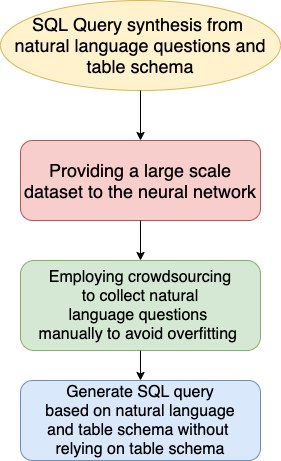
\includegraphics[width=0.4\textwidth]{pics/sqlnet/sqlnet.png}
\caption{SQLNet}
\label{fig:sqlnet}
\end{figure}

\subsubsection*{ Sketch-based query synthesis}

The token with the \$ sign represents an empty slot, and the token name represents the type of prediction. Tokens in bold represent SQL keywords such as SELECT, WHERE, etc.
\$AGG can be filled with either an empty token or one of the aggregation operators, such as SUM or MAX. Fill in the \$COLUMN and \$VALUE slots with the column name and substring of the question, respectively. The \$OP slot can be a value between \{=, \}. The notion \(...\)* uses a regular expression to indicate zero or more AND clauses.

\begin{figure}[htb]
    \centering
    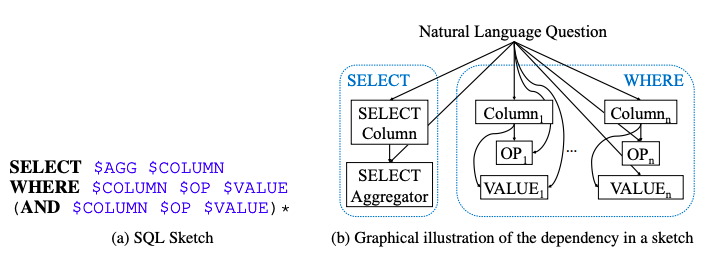
\includegraphics[width=0.8\textwidth]{pics/sqlnet/sketch-based.png}
    \caption{Sketch-based query synthesis}
    \label{fig:sketch-based}
\end{figure}

% bold text
\textbf{Column attention for sequence-to-set prediction}

Instead of producing a sequence of column names, sequence-to-set prediction predicts the names of the columns of interest.
Based on column names, column attention is part of the generic attention mechanism for computing the feature attention map on a question.

\textbf{Predicting WHERE and SELECT clause}
\begin{itemize}
    \item One of the most challenging tasks in Text2SQL is predicting the WHERE clause.
    \item According to SQL sketch, SQLNet finds the columns that appear in the WHERE clause and predicts the OP slots and value for each column.
    \item It is predicted that the OP slot will be filled with one of the three classes {<,>,=}, and the VALUE slot will be filled with the substring from the natural language question.
    \item In SELECT clauses, columns are named, and aggregator functions are specified, such as count, sum, max, etc. There is only one difference between SELECT and WHERE: the column name. There is only one column selected in SELECT.


In the WikiSQL test set, SQLNet accuracy is 64.4%, and in the SPIDER test set, it is around 12.4%.

\begin{figure}[htb]
    \centering
    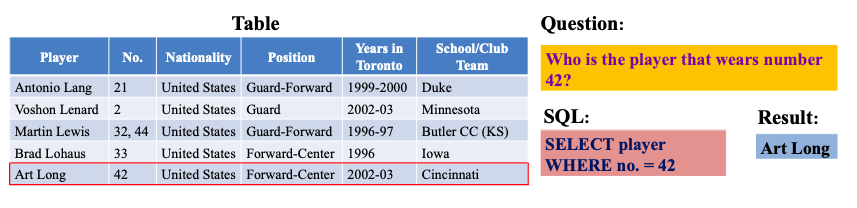
\includegraphics[width=0.8\textwidth]{pics/sqlnet/sqlnet-task.png}
    \caption{An example of a query executed by SQLNet on WikiSQL}
    \label{fig:sqlnet-task}
\end{figure}
\subsection*{SyntaxSQLNet}
% [2] Yu, Tao, et al. “Syntaxsqlnet: Syntax tree networks for the complex and cross-domain text-to-SQL task.” arXiv preprint arXiv:1810.05237 (2018).

\begin{itemize}
    \item The main goal of developing the SyntaxSQLNet model was to generate complex SQL queries with multiple clauses and generalize them to new databases.
    \item The model is based on a syntax tree network to address complex and cross-domain queries. The encoders are table-aware, and the decoders have a history of the SQL generation path.
    \item With a massive 7.3\% improvement in accuracy, SyntaxSQLNet outperformed previous models, such as SQLNet, on the SPIDER dataset.
\end{itemize}


\begin{figure}[htb]
    \centering
    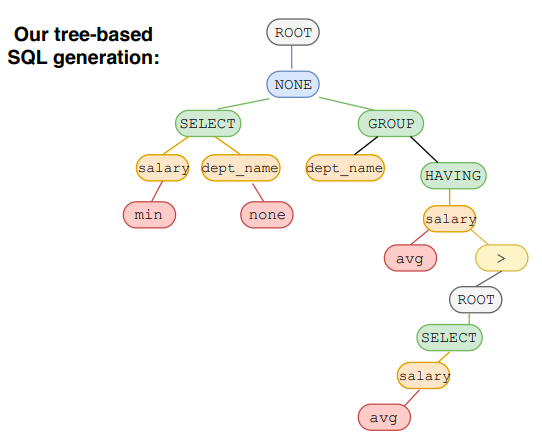
\includegraphics[width=0.8\textwidth]{pics/SyntaxSQLNet/Tree-based.png}
    \caption{Tree-based SQL generator in SyntaxSQLNet}
    \label{fig:tree-based}
\end{figure}

\begin{itemize}
    \item A cross-domain data augmentation technique further improves accuracy by generating more variance during training.
    \item Below is a chart showing the various modules and their functions.
\end{itemize}

\begin{figure}[htb]
    \centering
    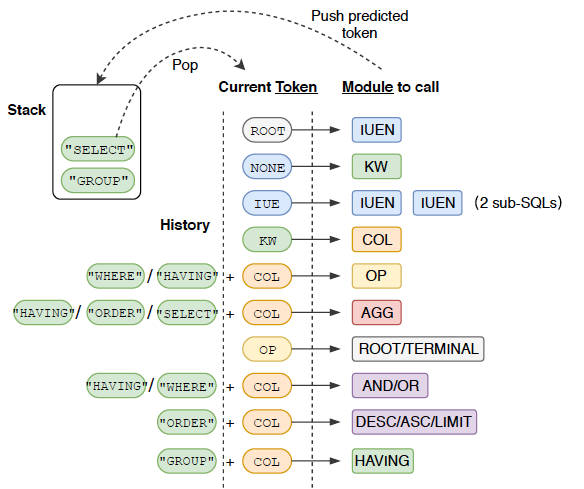
\includegraphics[width=0.8\textwidth]{pics/SyntaxSQLNet/Grammar.png}
    \caption{Modules defined in SyntaxSQLNet model}
    \label{fig:grammar}
\end{figure}


\textbf{SQL Grammar and Attention Mechanism}

\begin{itemize}
    \item In order to enable the decoder to handle complex queries, SQL grammar is used. At each step of recursive decoding, it determines which module to invoke.
    \item Predicting the next SQL token is also based on the history of SQL path generation and current SQL tokens.
    \item The attention mechanism is also used to encode the question representation. Attention also applies to SQL path history encoding.
\end{itemize}

\begin{figure}[htb]
    \centering
    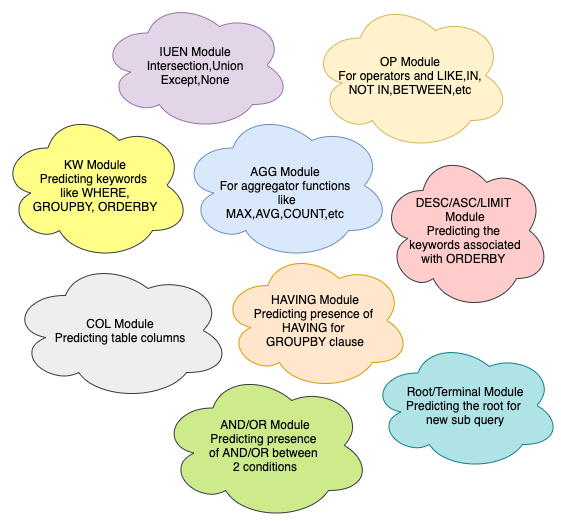
\includegraphics[width=0.8\textwidth]{pics/SyntaxSQLNet/Modules.png}
    \caption{Modules and SQL Grammar used in the decoding process}
    \label{fig:modules}
\end{figure}


\textbf{Data Augmentation}

\begin{itemize}
    \item Despite SPIDER's large dataset, it lacks complex queries.
    \item For proper generalization, cross-domain datasets are used for data augmentation.
    \item Various training databases of the SPIDER dataset are used to prepare a list of patterns for natural language questions and corresponding SQL queries.
\end{itemize}

The SPIDER model using syntaxSQLNet decoding history reaches 27.2\% accuracy.


Compared to previous models, such as SQLNet, the accuracy increased by 15\%.
\subsection*{GrammarSQL}
% \cite [3] Xu, Xiaojun, Chang Liu, and Dawn Song. “Sqlnet: Generating structured queries from natural language without reinforcement learning.” arXiv preprint arXiv:1711.04436 (2017).

Sequence-to-sequence models for neural text-to-SQL typically perform token-level decoding and do not consider generating SQL hierarchically.

\begin{itemize}
    \item [3] proposes a grammar-based model for reducing the complexity of text2SQL tasks involving hierarchical grammars.
    \item The authors introduce schema-dependent grammar with minimal over-generation.
    \item The grammar developed in [3] covers 98% of the instances in ATIS and SPIDER datasets.
\end{itemize}

\textbf{SQL Grammar}

\begin{itemize}
    \item The shallow parsing expression grammar aims to capture as little SQL as possible to cover most instances in the dataset.
    \item In order to ensure consistency of table, column, and value references in SQL, the authors added non-terminals to context-free grammar.
    \item They use runtime constraints during decoding to ensure that only valid programs can be used to join different tables in DB together using a foreign key.
\end{itemize}

\textbf{Few details on the proposed model}

\begin{itemize}
    \item As an input, the proposed model takes an utterance of natural language, a database, and grammar about that utterance.
    \item String matching heuristics are applied after taking the input to link words in the input to identifiers or tokens in the database.
    \item Afterward, the bidirectional LSTM receives a concatenated string of the learned word and the link embeddings for each token.
    \item Using the attention mechanism, the decoder builds up the SQL query iteratively on the input sequence.
    \item Database identifiers in natural language questions and SQL queries are also anonymized.
\end{itemize}

\begin{figure}[htb]
    \centering
    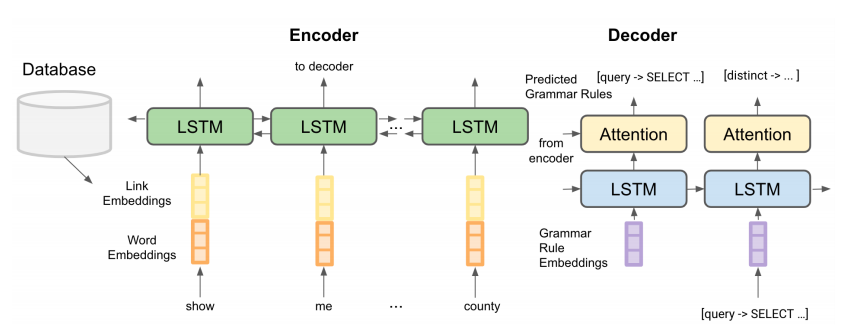
\includegraphics[width=0.8\textwidth]{pics/GrammarSQL.png}
    \caption{Structure of the proposed model}
    \label{fig:GrammarSQL}
\end{figure}


On ATIS and SPIDER datasets, the GrammarSQL model was evaluated. By 14%, it outperformed SyntaxSQLNet, the previous SOTA model.
% [1] Guo, Jiaqi, et al. “Towards complex text-to-SQL in the cross-domain database with intermediate representation.” arXiv preprint arXiv:1905.08205 (2019).

\subsection*{IRNet}

\begin{itemize}
    \item In Text2SQL tasks, the Intermediate Representation Network (IRNet) addresses two main challenges.
    \item Among the challenges are mismatches between natural language intents and predicting columns resulting from a more significant number of out-of-domain words.
    \item Instead of synthesizing SQL queries end-to-end, IRNet decomposes natural language into three phases.
    \item Schema linking is performed over a database schema and a question during the first phase.
    \item IRNet uses SemQL to bridge the gap between SQL and natural language.
    \item It includes a Natural Language (NL) encoder, a Schema Encoder, and a Decoder.
\end{itemize}

\begin{figure}[htb]
    \centering
    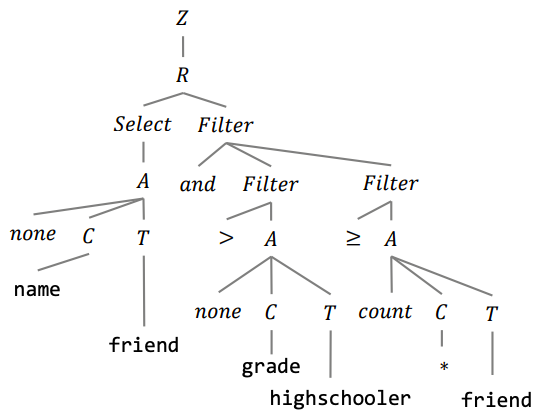
\includegraphics[width=0.8\textwidth]{pics/IRNet/illustrative_SemSQL}
    \caption{An illustrative example of SemSQL from [1]}
    \label{fig:illustrative_SemSQL}
\end{figure}

\begin{figure}[htb]
    \centering
    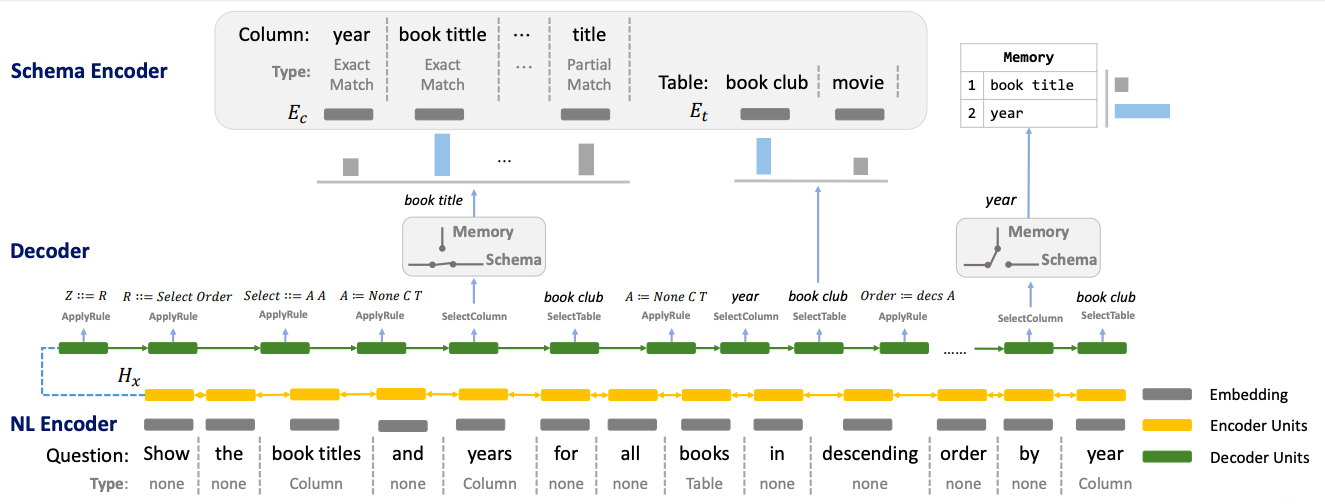
\includegraphics[width=0.8\textwidth]{pics/IRNet/overview}
    \caption{An overview of the neural model proposed in [1]}
    \label{fig:overview}
\end{figure}

\begin{itemize}
    \item The model provides different functions to accomplish Text2SQL tasks.
    \item Natural language is encoded into an embedding vector by the NL encoder. By using a bi-directional LSTM, these embedding vectors are used to construct hidden states.
    \item A schema encoder takes a database schema as input and outputs representations for columns and tables.
    \item Using a context-free grammar, the decoder synthesizes SemQL queries.
    \item On the SPIDER dataset, IRNet performs 46.7\% better than previous benchmark models by 19%.
    \item The accuracy of 54.7\% is achieved by combining IRNet with BERT.
\end{itemize}

\begin{figure}[htb]
    \centering
    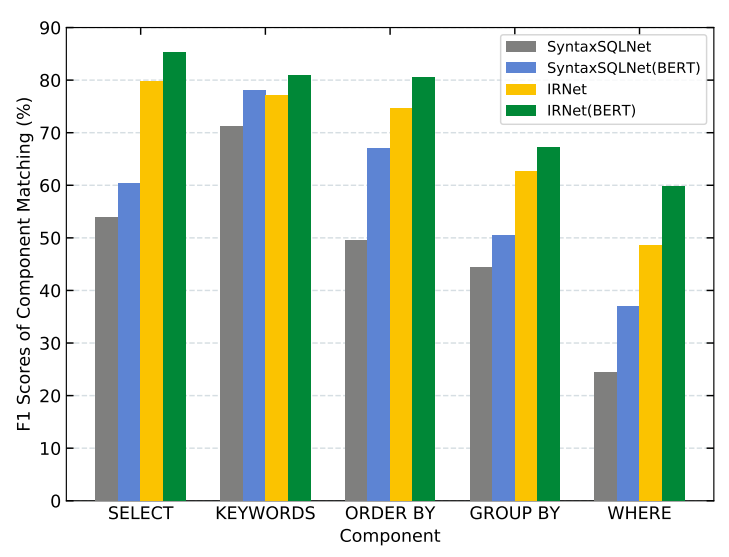
\includegraphics[width=0.8\textwidth]{pics/IRNet/f1}
    \caption{F1 scores of component matching of SyntaxSQLNet, SyntaxSQLNet(BERT), IRNet and IRNet(BERT) on the test set from [1]}
    \label{fig:f1}
\end{figure}

\subsection*{EditSQL}

\begin{itemize}
    \item EditSQL focuses on text-to-SQL tasks that are context-dependent across domains.
    \item It exploits the fact that adjacent natural language questions are dependent on one another and that corresponding SQL queries overlap.
    \item To improve the generation quality, they edit the previously predicted query.
    \item The editing mechanism reuses generation results at the token level based on SQL input sequences.
    \item An utterance-table encoder and a table-aware decoder are utilized to incorporate the context of the natural language and the schema when dealing with complicated tables in different domains.
\end{itemize}

\begin{figure}[htb]
    \centering
    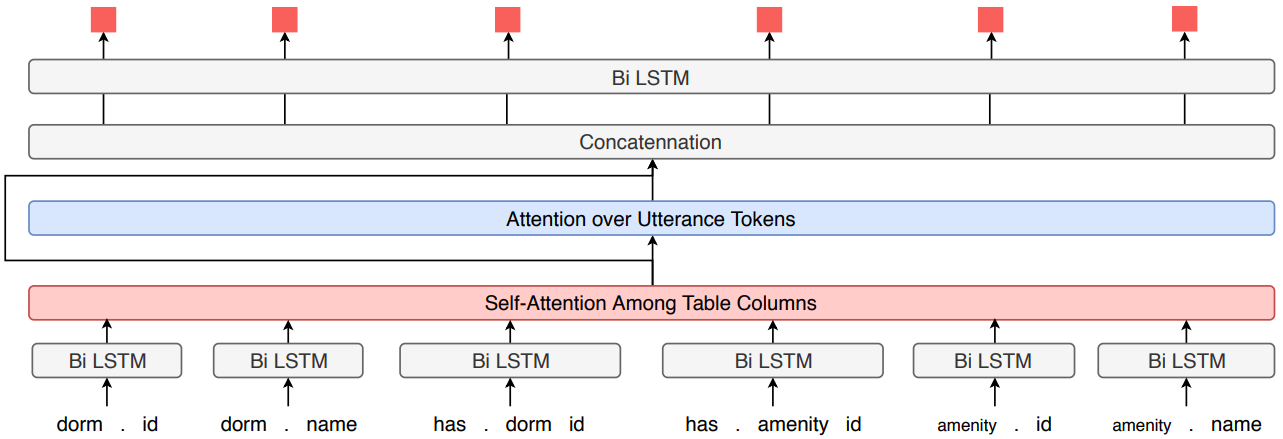
\includegraphics[width=0.8\textwidth]{pics/EditSQL/Table.png}
    \caption{The model architecture of EditSQL from \cite{DBLP:journals/corr/abs-1909-00786}}
    \label{fig:EditSQL}
\end{figure}


\begin{itemize}
    \item User utterances and table schemas are encoded by the utterance-table encoder. Tokens of utterances are encoded using a bi-LSTM.
    \item To determine the most relevant columns, Attention weighed an average of column header embedding is applied to each token.
\end{itemize}

\begin{figure}[htb]
    \centering
    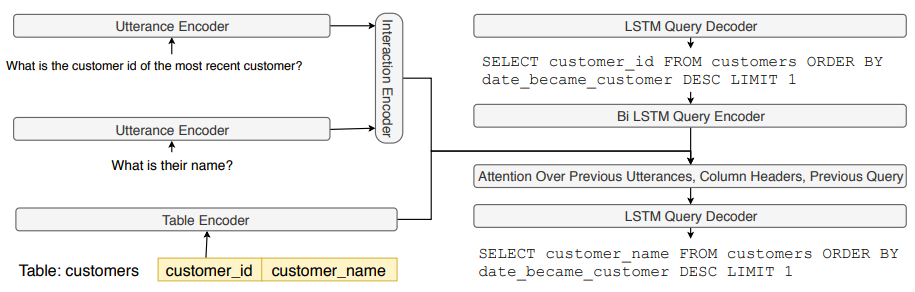
\includegraphics[width=0.8\textwidth]{pics/EditSQL/model.png}
    \caption{An example of user utterance and column headers and Utterance Encoder from \cite{DBLP:journals/corr/abs-1909-00786}}
    \label{fig:EditSQL_model}
\end{figure}

\begin{itemize}
    \item To capture the relationship between table schema and utterance, an attention layer is incorporated.
    \item The utterance-level encoder is built on top of an interaction-level decoder in order to capture information across utterances.
    \item LSTM decoding is used to generate SQL queries by incorporating interaction history, table schema, and user utterances.
\end{itemize}

\begin{figure}[htb]
    \centering
    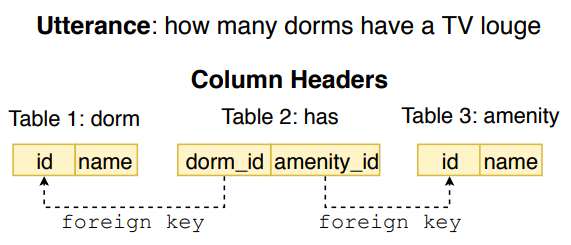
\includegraphics[width=0.5\textwidth]{pics/EditSQL/example.png}
    \caption{Table Encoder from \cite{DBLP:journals/corr/abs-1909-00786}}
    \label{fig:EditSQL_example}
\end{figure}

\begin{itemize}
    \item The model is evaluated on the SParC dataset, a large cross-domain context-dependent semantic parsing dataset derived from SPIDER.
    \item In both SPIDER and SParC, the model outperforms the previous state of the art model, IRNet.
    \item In cross-domain text2SQL generation, the model achieves 32.9\% accuracy. A 53.4\% improvement in accuracy can be achieved by using BERT embedding.
\end{itemize}

\subsection*{RAT-SQL}

\begin{figure}[htb]
    \centering
    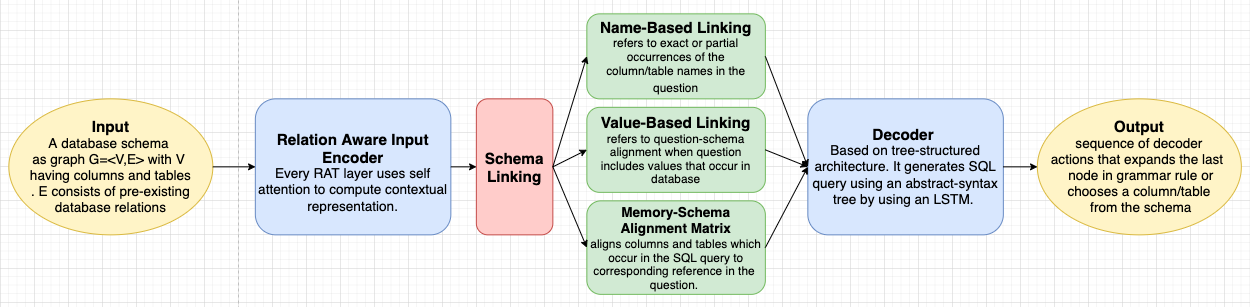
\includegraphics[width=0.8\textwidth]{pics/RAT-SQL/flow.png}
    \caption{A flow chart of RAT-SQL model}
    \label{fig:RAT-SQL-flow}
\end{figure}

\begin{itemize}
    \item A major challenge in translating natural language queries into SQL queries is generalizing them to unknown database schemas.
    \item As part of the generalisation, it is necessary to encode database relations in an accessible way and model alignment between relevant database columns in the query.
    \item Within a text2SQL encoder, the proposed framework leverages the relation-aware self-attention mechanism to encode address schemas, represent features, and link schemas.
    \item Check out the flow chart below for an overview of RAT-SQL's encoder-decoder structure.
\end{itemize}

\begin{figure}[htb]
    \centering
    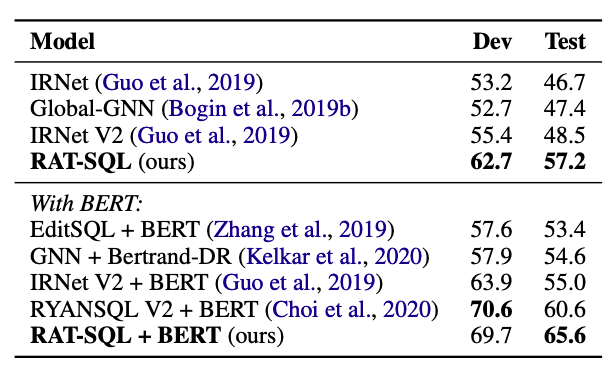
\includegraphics[width=0.4\textwidth]{pics/RAT-SQL/Accuracy.png}
    \caption{Accuracy on the Spider development and test sets, compared to the other approaches at the top of the dataset leaderboard as of May 1st, 2020 from \cite{wang_rat-sql_2021}}
    \label{fig:RAT-SQL-Accuracy}
\end{figure}

On the SPIDER dataset, RAT-SQL achieves 57.2\% accuracy, an improvement of 8.7\% over previous benchmark models.

\begin{figure}[htb]
    \centering
    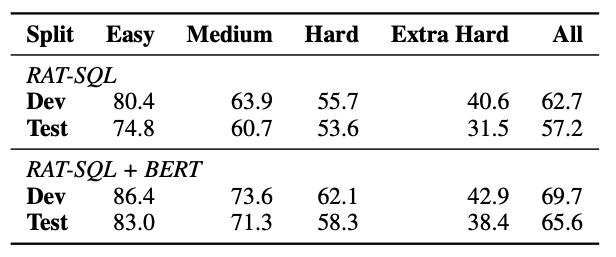
\includegraphics[width=0.4\textwidth]{pics/RAT-SQL/Accuracy2.png}
    \caption{Accuracy on the Spider development and test sets, by difficulty from \cite{wang_rat-sql_2021}}
    \label{fig:RAT-SQL-Accuracy2}
\end{figure}

With RAT-SQL, 65.6\% accuracy can be achieved by combining BERT with RAT-SQL.

\input{inc/models/BRIDGE}
\subsection*{Picard}

Picard\cite{scholak_picard_2021} stands for "Parsing Incrementally for Constrained Auto-Regressive Decoding.". It can be used with any existing language model decoder or vocabulary based on auto-regressive language modeling.

As an optional feature, Picard can be enabled at inference time and is absent from pre-training or fine-tuning. In the case of text-to-SQL translation, Picard operates directly on the output of the language model.
Picard demonstrates state-of-the-art performance on challenging Spider and CoSQL text-to-SQL translation tasks.

Picard warps model prediction scores and integrates trivially with existing greedy and beam search algorithms. In addition to the token ids of the current hypothesis, the model's language modeling head also predicts the log-softmax scores for each vocabulary token. Additionally, Picard has access to SQL schema information, including table and column names and which column resides in which table.

% \begin{itemize}
%   \item Seq2SQL and SQLNet will perform encoding using LSTM/Bi-LSTM and decode using classification and Pointer Network.
%   \item SQLova and HydraNet encode natural language queries through a language model and decode them through the Natural Language-to-SQL layer, converting them to SQL grammars. Going a little further, SQLova was the first to use a language model as an encoder, encode questions and columns, and then predict queries.
%   \item HydraNet uses BERT's token to rank columns one by one to fill in the slots of the SQL Query statement. Brief description of the BERT will be given in our final report.
%   \item Since the SPIDER dataset used for RAT-SQL and BRIDGE is a Multi-Table, it is necessary to understand the Schema's relationship to the question and its internal relationships, for which Schema Linking and Encoding are applied, and decoders such as SemQL are utilized.
%   \item RAT-SQL reflects the schema information into the encoding and decoding with SemQL, including the relationships extracted from the question-scheme contextualized graph in Self-Attention.
%   \item BRIDGE achieves Schema Linking by including the Schema's Table and Column Name and Value in the Encoding and utilizes the Pointer Generator Network as the Decoder.
%   \item PICARD proposes a new method for simple and effective constrained decoding with large pre-trained language models.
%         On both the SPIDER cross-domain and cross-database Text-to-SQL dataset and the CoSQL SQL-grounded dialog state tracking dataset, we find that the PICARD decoding method not only significantly improves the performance of fine-tuned unmodified T5 models but it also lifts a T5-3B model to state-of-the-art results on the established exact-match and execution accuracy metrics.
% \end{itemize}